\documentclass[a4paper]{article}
\usepackage{ctex}
\usepackage{enumitem}
\usepackage{multirow}
\usepackage{fancyhdr}
\usepackage{amsmath}
\usepackage{parskip}
\usepackage{float}
\usepackage{listings}
\usepackage{hyperref}
\usepackage{tikz, pgfplots}

\lstset{basicstyle=\ttfamily,breaklines=true,showstringspaces=false}

\setlength{\parskip}{6pt}

\pagestyle{headings}

\begin{document}
\title{文本情感分类实验}
\author{梁业升 2019010547(计03)}

\maketitle

本实验实现及原理参考了 \url{https://github.com/bentrevett/pytorch-sentiment-analysis}。

\section*{实验环境}

系统:\texttt{macOS 12.3.1}\\
环境:\texttt{Python 3.9.10}

\section{模型概述}

\subsection{RNN}

\begin{figure}[H]
    \centering
    \includegraphics[width=0.9\textwidth]{assets/rnn.png}
    \caption{RNN}
\end{figure}

RNN 以1个词$x$和一个隐藏状态$h_0$作为输入,并产生下一个隐藏状态$h$。我们对词序列$X=\{x_1,\ldots,x_T\}$循环使用 RNN,将当前词$x_t$以及前一个隐藏状态$h_{t-1}$作为输入,产生隐藏状态$h_t$,即

\begin{equation}
    h_t=\textrm{RNN}(x_t,h_{t-1})
\end{equation}

最后一个隐藏状态$h_t$经过一个全连接层后即可得到预测值。

RNN有多个变种,如双向RNN:

\begin{figure}[H]
    \centering
    \includegraphics[width=0.9\textwidth]{assets/bi-rnn.png}
    \caption{双向RNN}
\end{figure}

多层RNN:

\begin{figure}[H]
    \centering
    \includegraphics[width=0.9\textwidth]{assets/mul-rnn.jpg}
    \caption{多层RNN}
\end{figure}

标准的RNN有梯度消失的问题。我们使用如下图所示的LSTM解决此问题:

\begin{figure}[H]
    \centering
    \includegraphics[width=0.9\textwidth]{assets/lstm.png}
    \caption{LSTM}
\end{figure}

与标准RNN相比,LSTM多了一个额外的状态$c$:

\begin{equation}
    (h_t,c_t)=\textrm{LSTM}(x_t,h_{t-1},c_{t-1})
\end{equation}

LSTM使用多个门控制信息流入和流出$c$,以达到“记忆”的功能。

\begin{figure}[H]
    \centering
    \includegraphics[width=0.9\textwidth]{assets/lstm-cell.png}
    \caption{LSTM cell}
\end{figure}

\subsection{CNN}

将词向量纵向排列,得到一个二维的输入。

\begin{figure}[H]
    \centering
    \includegraphics[width=0.9\textwidth]{assets/cnn-1.png}
    \caption{卷积层}
\end{figure}

输入经过卷积层后得到一个一维或多维的向量。我们对其进行最大池化:

\begin{figure}[H]
    \centering
    \includegraphics[width=0.9\textwidth]{assets/cnn-2.png}
    \caption{最大池化}
\end{figure}

为了提取不同长度的词的组合的特征(如“非常 好”和“非常”“好”),我们使用多个大小(如1,2,3)的卷积核,并将进行最大池化的结果拼接在一起,通过全连接层产生输出。

\subsection{模型优化}

为缓解过拟合的问题,我们在模型的全连接层前加上 Dropout 层,即随机将一些神经元输出置0。

\section{实验结果}

我们用3个标准来评价模型的效果:测试集上的准确率(Accuracy)、测试集上的F1-Score,以及训练一个周期需要的时间。

训练在 \href{https://colab.research.google.com/}{Google Colab} 上进行。由于以下针对不同参数的实验并不在同一时间进行,而平台在不同时间的可用资源情况不同,因此不同实验对应的训练用时不具有可比性。

\subsection{LSTM}

我们考察3个超参数对模型效果的影响:层数\texttt{layer\_num}、Dropout层的丢弃概率\texttt{dropout\_rate}和一次处理的输入数量\texttt{batch\_size}。

\subsubsection{LSTM层数}

固定 \texttt{dropout\_rate = 0},\texttt{batch\_size = 64}。实验结果如下:

\begin{figure}[H]
    \centering
    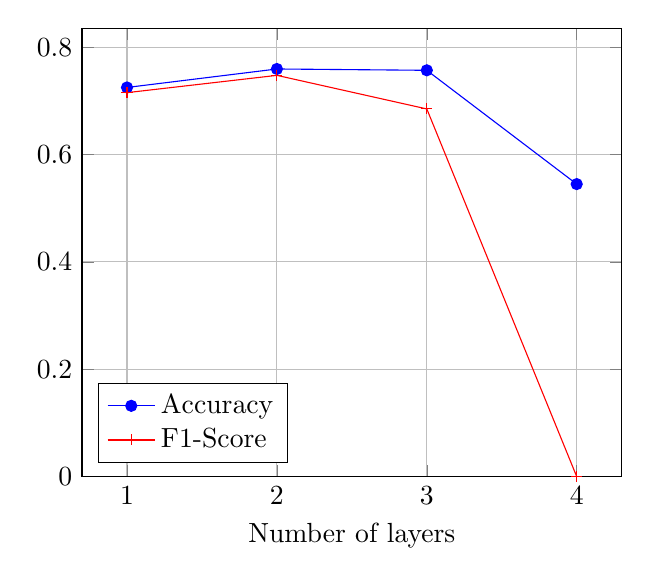
\begin{tikzpicture} 
        \begin{axis}[
            legend cell align=left,
            legend pos=south west,
            xlabel={Number of layers}, 
            xtick=data,
            ymin=0,
            grid=both
        ] 
        \addplot [blue, mark=*] coordinates {
            (1, 0.7250212530295054)
            (2, 0.7594600319862366)
            (3, 0.757)
            (4, 0.5449617306391398)
        };\addlegendentry{Accuracy}
        \addplot [red, mark=+] coordinates {
            (1, 0.7153478562831879)
            (2, 0.7475786606470743)
            (3, 0.685)
            (4, 0)
        };\addlegendentry{F1-Score}
        \end{axis} 
    \end{tikzpicture}
\end{figure}

\begin{figure}[H]
    \centering
    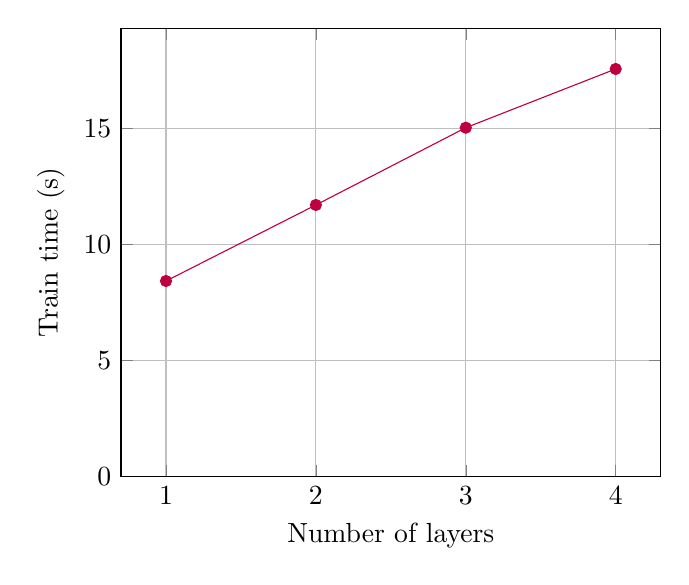
\begin{tikzpicture} 
        \begin{axis}[
            legend cell align=left,
            legend pos=south west,
            xlabel={Number of layers},
            ylabel={Train time (s)}, 
            xtick=data,
            ymin=0,
            grid=both
        ] 
        \addplot [purple, mark=*] coordinates {
            (1, 8.431526548)
            (2, 11.7102487087)
            (3, 15.0419525933)
            (4, 17.5740004645)
        };
        \end{axis} 
    \end{tikzpicture}
\end{figure}

可见,双层LSTM比单层LSTM在效果上有略微的提高,但极其有限;当层数继续增加时,效果反而会有明显的下降;在层数为4时模型几乎完全无法训练,推测是出现了梯度消失的问题。同时,训练时间相对层数大约线性增长。因此,增加层数并不能起到明显的作用,反而会增加训练时间。

\subsubsection{Dropout概率}

固定 \texttt{layer\_num = 2},\texttt{batch\_size = 64}。实验结果如下:

\begin{figure}[H]
    \centering
    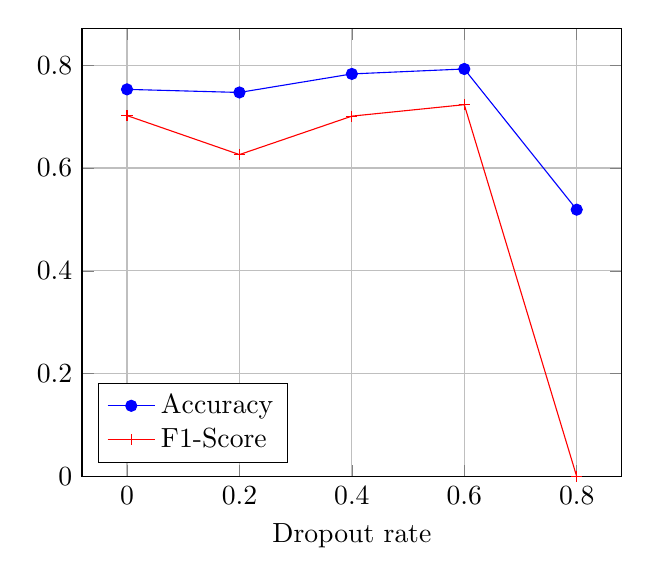
\begin{tikzpicture} 
        \begin{axis}[
            legend cell align=left,
            legend pos=south west,
            xlabel={Dropout rate}, 
            ymin=0,
            grid=both
        ] 
        \addplot [blue, mark=*] coordinates {
            (0, 0.7528698941071829)
            (0.2, 0.7468643685181936)
            (0.4, 0.7828975319862366)
            (0.6, 0.7925170063972473)
            (0.8, 0.5189200639724731)
        };\addlegendentry{Accuracy}
        \addplot [red, mark=+] coordinates {
            (0, 0.7019334187110265)
            (0.2, 0.6260340809822083)
            (0.4, 0.70081893603007)
            (0.6, 0.7230925659338633)
            (0.8, 0.0)
        };\addlegendentry{F1-Score}
        \end{axis} 
    \end{tikzpicture}
\end{figure}

\begin{figure}[H]
    \centering
    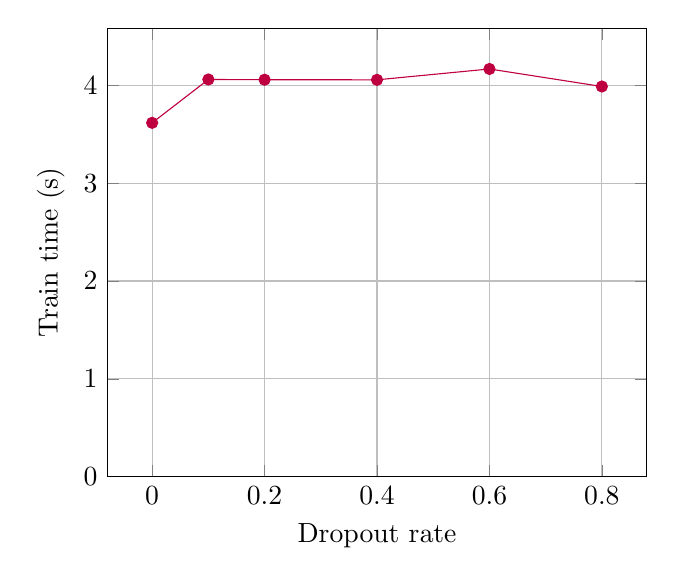
\begin{tikzpicture} 
        \begin{axis}[
            legend cell align=left,
            legend pos=south west,
            xlabel={Dropout rate},
            ylabel={Train time (s)}, 
            ymin=0,
            grid=both
        ] 
        \addplot [purple, mark=*] coordinates {
            (0, 3.6182848394)
            (0.1, 4.0617841542)
            (0.2, 4.0593671918)
            (0.4, 4.0582030416)
            (0.6, 4.1691816539)
            (0.8, 3.9900371671)
        };
        \end{axis} 
    \end{tikzpicture}
\end{figure}

相比不使用 Dropout 层,当随机丢弃的概率为0.2时,模型效果略有下降;概率为0.4、0.6时,模型效果有所上升;概率为0.8时,模型几乎无法训练。实验结果表明,经过对参数进行一定比例的丢弃,可以在一定程度上缓解过拟合的问题。

\subsubsection{Batch size}

固定 \texttt{layer\_num = 2},\texttt{dropout\_rate = 0}。实验结果如下:

\begin{figure}[H]
    \centering
    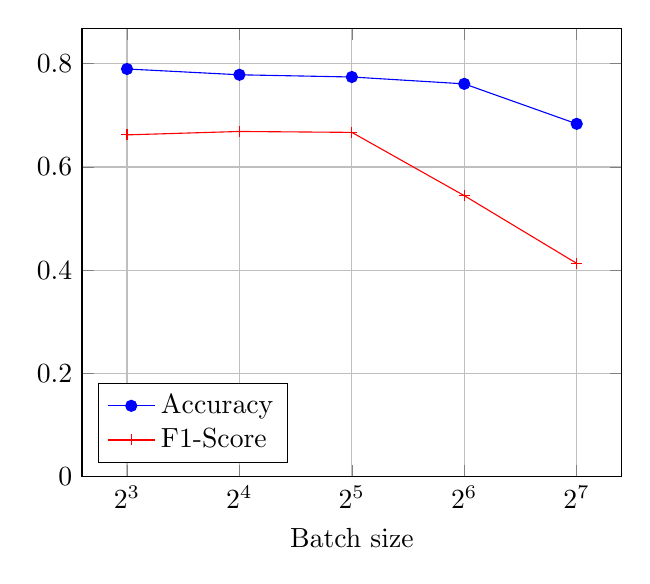
\begin{tikzpicture} 
        \begin{axis}[
            legend cell align=left,
            legend pos=south west,
            xlabel={Batch size}, 
            xmode=log,
            log basis x={2},
            ymin=0,
            grid=both
        ] 
        \addplot [blue, mark=*] coordinates {
            (8, 0.7898936170212766)
            (16, 0.7786458333333334)
            (32, 0.7743566185235977)
            (64, 0.7610544164975485)
            (128, 0.6835822264353434)
        };\addlegendentry{Accuracy}
        \addplot [red, mark=+] coordinates {
            (8, 0.6621862947940826)
            (16, 0.6688011276225249)
            (32, 0.667030523220698)
            (64, 0.544399564464887)
            (128, 0.4131622016429901)
        };\addlegendentry{F1-Score}
        \end{axis} 
    \end{tikzpicture}
\end{figure}

\begin{figure}[H]
    \centering
    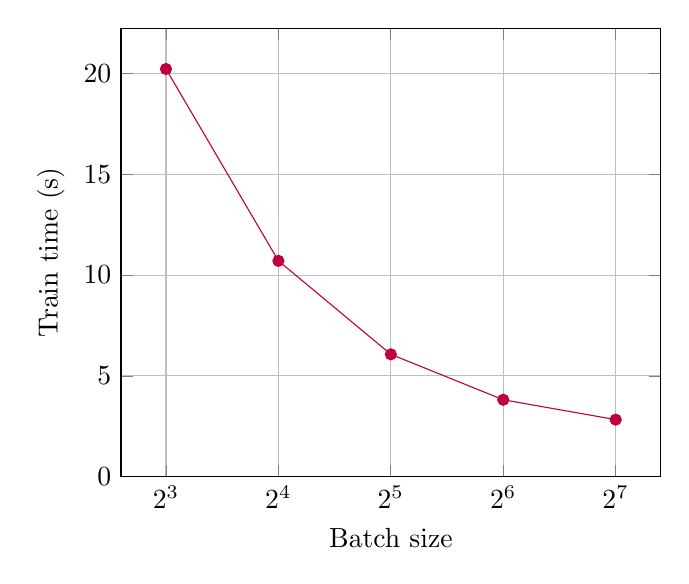
\begin{tikzpicture} 
        \begin{axis}[
            legend cell align=left,
            legend pos=south west,
            xlabel={Batch size}, 
            ylabel={Train time (s)}, 
            xmode=log,
            log basis x={2},
            ymin=0,
            grid=both
        ] 
        \addplot [purple, mark=*] coordinates {
            (8, 20.2280266626)
            (16, 10.7058820838)
            (32, 6.0664029348)
            (64, 3.8107119582)
            (128, 2.8250296879)
        };
        \end{axis} 
    \end{tikzpicture}
\end{figure}

模型效果总体上与单批处理的数量呈负相关,而训练时间随单批处理的数量呈负相关。这是容易理解的,因为更粗粒度的训练所保留的训练集的细节更少,因此准确率更低;同时因为其前向和反向传播的次数更少,因此用时更少。

由实验结果不难得到,在实验的条件下,以32为单批处理的数量较为合适。

\subsection{CNN}

我们考察3个超参数对模型效果的影响:卷积层输出通道数\texttt{channel\_num}、Dropout层的丢弃概率\texttt{dropout\_rate}和一次处理的输入数量\texttt{batch\_size}。

\subsubsection{输出通道数}

固定 \texttt{dropout\_rate = 0},\texttt{batch\_size = 64}。实验结果如下:

\begin{figure}[H]
    \centering
    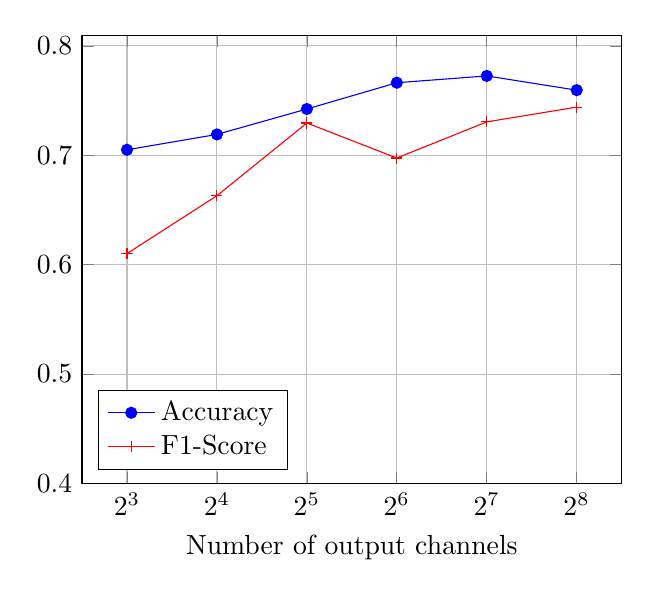
\begin{tikzpicture} 
        \begin{axis}[
            legend cell align=left,
            legend pos=south west,
            xlabel={Number of output channels}, 
            ymin=0.4,
            xmode=log,
            log basis x={2},
            grid=both
        ] 
        \addplot [blue, mark=*] coordinates {
            (8, 0.704985111951828)
            (16, 0.7190157274405161)
            (32, 0.7422406474749247)
            (64, 0.7662627498308817)
            (128, 0.7724808653195699)
            (256, 0.7594600319862366)
        };\addlegendentry{Accuracy}
        \addplot [red, mark=+] coordinates {
            (8, 0.6101107796033224)
            (16, 0.662991484006246)
            (32, 0.7294404109319051)
            (64, 0.6974337746699651)
            (128, 0.7304725547631582)
            (256, 0.7439627250035604)
        };\addlegendentry{F1-Score}
        \end{axis} 
    \end{tikzpicture}
\end{figure}

\begin{figure}[H]
    \centering
    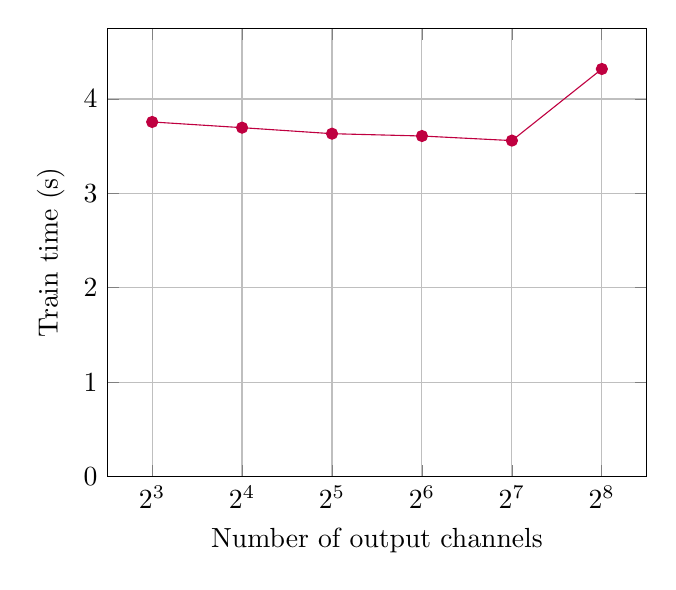
\begin{tikzpicture} 
        \begin{axis}[
            legend cell align=left,
            legend pos=south west,
            xlabel={Number of output channels},
            ylabel={Train time (s)}, 
            xmode=log,
            log basis x={2},
            ymin=0,
            grid=both
        ] 
        \addplot [purple, mark=*] coordinates {
            (8, 3.7565025269985197)
            (16, 3.696005165576935)
            (32, 3.6322301983833314)
            (64, 3.607688343524933)
            (128, 3.559057152271271)
            (256, 4.317773592472077)
        };
        \end{axis} 
    \end{tikzpicture}
\end{figure}

\subsubsection{Dropout概率}

固定 \texttt{channel\_num = 100},\texttt{batch\_size = 64}。实验结果如下:

\begin{figure}[H]
    \centering
    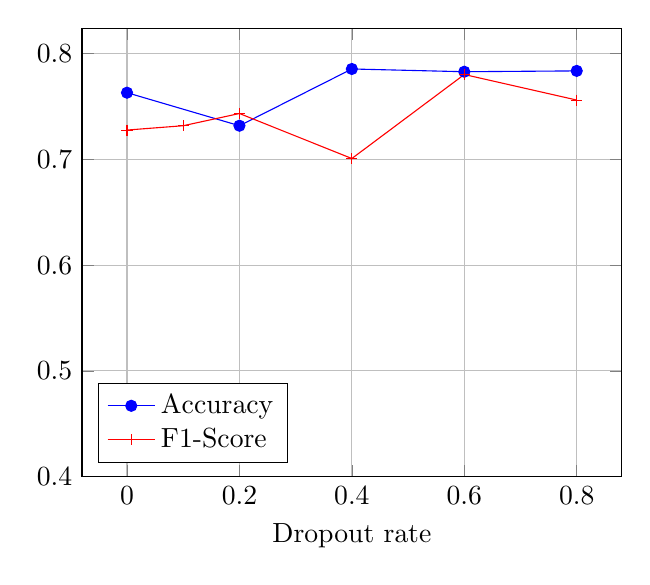
\begin{tikzpicture} 
        \begin{axis}[
            legend cell align=left,
            legend pos=south west,
            xlabel={Dropout rate}, 
            ymin=0.4,
            grid=both
        ] 
        \addplot [blue, mark=*] coordinates {
            (0, 0.7630739808082581)
            (0.2, 0.7318239808082581)
            (0.4, 0.7855016986529032)
            (0.6, 0.7828975319862366)
            (0.8, 0.7836947242418925)
        };\addlegendentry{Accuracy}
        \addplot [red, mark=+] coordinates {
            (0, 0.7277275423208872)
            (0.1, 0.731833428144455)
            (0.2, 0.7433765232563019)
            (0.4, 0.70081893603007)
            (0.6, 0.7802693446477255)
            (0.8, 0.7561041414737701)
        };\addlegendentry{F1-Score}
        \end{axis} 
    \end{tikzpicture}
\end{figure}

\begin{figure}[H]
    \centering
    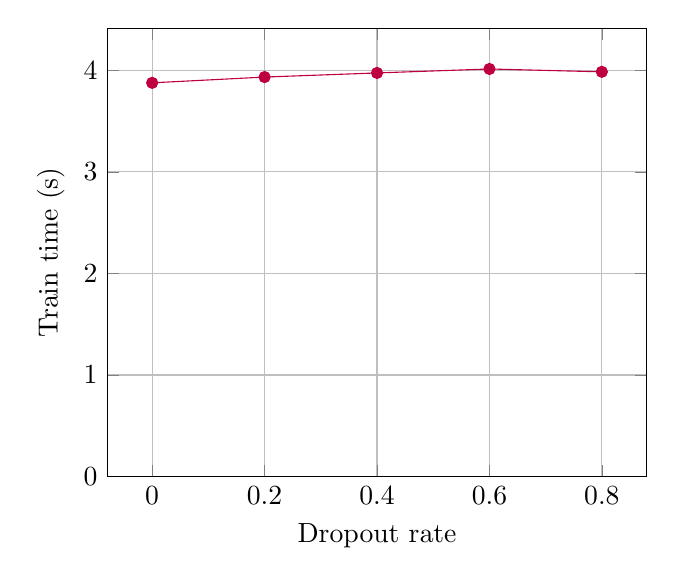
\begin{tikzpicture} 
        \begin{axis}[
            legend cell align=left,
            legend pos=south west,
            xlabel={Dropout rate},
            ylabel={Train time (s)}, 
            ymin=0,
            grid=both
        ] 
        \addplot [purple, mark=*] coordinates {
            (0, 3.8758679211139677)
            (0.2, 3.932650017738342)
            (0.4, 3.9732058167457582)
            (0.6, 4.012242740392685)
            (0.8, 3.984130722284317)
        };
        \end{axis} 
    \end{tikzpicture}
\end{figure}

\subsubsection{Batch size}

固定 \texttt{layer\_num = 2},\texttt{dropout\_rate = 0}。实验结果如下:

\begin{figure}[H]
    \centering
    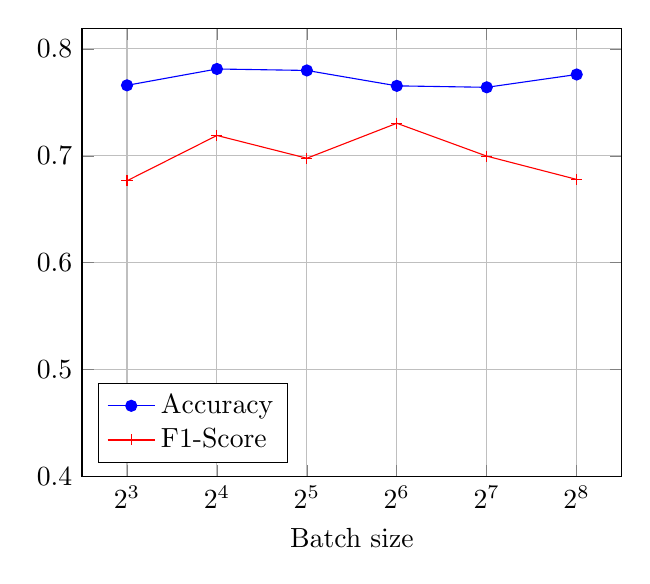
\begin{tikzpicture} 
        \begin{axis}[
            legend cell align=left,
            legend pos=south west,
            xlabel={Batch size}, 
            xmode=log,
            ymin=0.4,
            log basis x={2},
            grid=both
        ] 
        \addplot [blue, mark=*] coordinates {
            (8, 0.7659574468085106)
            (16, 0.78125)
            (32, 0.7798713246981303)
            (64, 0.7654655575752258)
            (128, 0.7641039888064066)
            (256, 0.7760992646217346)
        };\addlegendentry{Accuracy}
        \addplot [red, mark=+] coordinates {
            (8, 0.6766814817773535)
            (16, 0.7190621569752693)
            (32, 0.6977513631184896)
            (64, 0.7304713030656179)
            (128, 0.6997187336285909)
            (256, 0.6779427528381348)
        };\addlegendentry{F1-Score}
        \end{axis} 
    \end{tikzpicture}
\end{figure}

\begin{figure}[H]
    \centering
    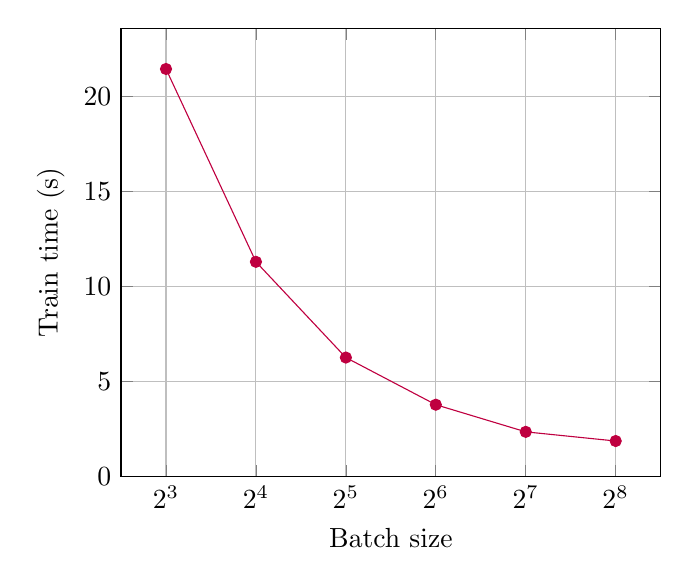
\begin{tikzpicture} 
        \begin{axis}[
            legend cell align=left,
            legend pos=south west,
            xlabel={Batch size}, 
            ylabel={Train time (s)}, 
            xmode=log,
            log basis x={2},
            ymin=0,
            grid=both
        ] 
        \addplot [purple, mark=*] coordinates {
            (8, 21.43460758924484)
            (16, 11.292743515968322)
            (32, 6.258250272274017)
            (64, 3.7781805813312532)
            (128, 2.350329279899597)
            (256, 1.8683703422546387)
        };
        \end{axis} 
    \end{tikzpicture}
\end{figure}
\end{document}
